\documentclass[11pt]{article}

\usepackage[utf8]{inputenc}
\usepackage[T1]{fontenc}
\usepackage[english]{babel}
\usepackage{graphicx}
\usepackage{amsmath,amssymb,amsthm,amsopn}
\usepackage{mathrsfs}
\usepackage{graphicx}
\usepackage{array}
\usepackage{makecell}


\usepackage{hyperref}
\hypersetup{
    colorlinks=true,
    linkcolor=blue,
    citecolor=red,
}

%\usepackage[top=1cm,bottom=1cm]{geometry}
%\usepackage{listings}
%\usepackage{xcolor}

\usepackage{tikz}

% Tikz style

\tikzset{round/.style={circle, draw=black, very thick, scale = 0.7}}
\tikzset{arrow/.style={->, >=latex}}
\tikzset{dashed-arrow/.style={->, >=latex, dashed}}

\newtheoremstyle{break}%
{}{}%
{\itshape}{}%
{\bfseries}{}%  % Note that final punctuation is omitted.
{\newline}{}

\newtheoremstyle{sc}%
{}{}%
{}{}%
{\scshape}{}%  % Note that final punctuation is omitted.
{\newline}{}

\theoremstyle{break}
\newtheorem{thm}{Theorem}[section]
\newtheorem{lm}[thm]{Lemma}
\newtheorem{prop}[thm]{Proposition}
\newtheorem{cor}[thm]{Corollary}

\theoremstyle{sc}
\newtheorem{exo}{Exercice}

\theoremstyle{definition}
\newtheorem{defi}[thm]{Definition}
\newtheorem{ex}[thm]{Example}

\theoremstyle{remark}
\newtheorem{rem}[thm]{Remark}

% Math Operators

\DeclareMathOperator{\Card}{Card}
\DeclareMathOperator{\Gal}{Gal}
\DeclareMathOperator{\Id}{Id}
\DeclareMathOperator{\Img}{Im}
\DeclareMathOperator{\Ker}{Ker}
\DeclareMathOperator{\Minpoly}{Minpoly}
\DeclareMathOperator{\Mod}{mod}
\DeclareMathOperator{\Ord}{Ord}
\DeclareMathOperator{\ppcm}{ppcm}
\DeclareMathOperator{\Tr}{Tr}
\DeclareMathOperator{\Vect}{Vect}

% Shortcuts

\newcommand{\dE}{\partial(E)}
\newcommand{\dF}{\partial(F)}
\newcommand{\dG}{\partial(G)}
\newcommand{\diff}{\mathop{}\!\mathrm{d}}
\newcommand{\eg}{\emph{e.g. }}
\newcommand{\emb}{\hookrightarrow}
\newcommand{\embed}[2]{\phi_{#1\hookrightarrow#2}}
\newcommand{\ent}[2]{[\![#1,#2]\!]}
\newcommand{\ie}{\emph{i.e. }}
\newcommand{\ps}[2]{\left\langle#1,#2\right\rangle}





\title{Lattices of compatibly embedded finite fields}
\author{}

\begin{document}
\maketitle
\begin{center}
  
    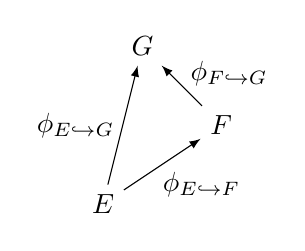
\begin{tikzpicture}
      \node (E) at (0, 0) {$E$}; 
      \node (F) at (1.5, 1) {$F$}; 
      \node (G) at (0.5, 2) {$G$}; 

      \draw[arrow] (E) -- (F);
      \draw[arrow] (E) -- (G);
      \draw[arrow] (F) -- (G);

      \node (f12) at (1.25, 0.25) {$\embed{E}{F}$};
      \node (f13) at (-0.35, 1) {$\embed{E}{G}$};
      \node (f23) at (1.6, 1.65) {$\embed{F}{G}$};
    \end{tikzpicture}

\end{center}

\section{Introduction}

Given two finite fields $E$ and $F$ with cardinalities $|E|=p^{m}$ and
$|F|=p^{n}$, we know that $E$ can be embedded in $F$ if and only if $m\,|\,n$.
In other words, $E$ is in that case isomorphic to a subfield $E'\subset F$ of $F$ with
cardinality $|E'|=p^{m}$. There are
$m=[E:\mathbb{F}_p]=|\Gal(E/\mathbb{F}_p)|$ disctinct embeddings from $E$ to
$F$ (the degree of $E$ over $\mathbb{F}_p$ will also be denoted by
$\partial(E)$). Indeed, the Galois group of the extension $E$ over $\mathbb{F}_p$ acts
on the embeddings. Given two different embeddings $\embed{E}{F}$ and
$\embed{E}{F}'$ and an element $x\in E$, the images $\embed{E}{F}(x)$ and
$\embed{E}{F}'(x)$ must be conjugates. As a result, there is no cannonical
embedding from $E$ to $F$. Furthermore, the proof of the fact that $E$ can be
embedded in $F$ if and only if $\dE\,|\,\dF$ is not constructive, so computing the
embedding is itself a challenging problem, and there exists a variety of
solutions.

In this document, we do not recall the embeddings algorithms, we often
consider them as black boxes that we use to construct embeddings between
finite fields, and we study the compatibility between these embeddings. Given
three finite fields $E$, $F$, and $G$, such that $\dE\,|\,\dF$ and $\dF\,|\,\dG$, and three embeddings
$\embed{E}{F}$, $\embed{F}{G}$, and $\embed{E}{G}$, we say that the
embeddings are \emph{compatible} if 
\[
  \embed{E}{G}=\embed{F}{G}\circ\embed{E}{F}.
\]
In other words, we want the diagram of Figure~\ref{fig:compatibility} to
commute. We also note $E\emb F$ if $E$ is explicitly embedded in $F$, \ie if
we have computed an embedding $\embed{E}{F}$.
\begin{figure}
  \centering
    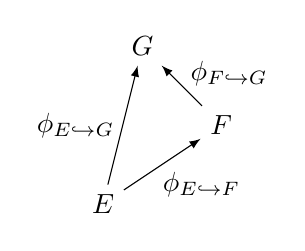
\begin{tikzpicture}
      \node (E) at (0, 0) {$E$}; 
      \node (F) at (1.5, 1) {$F$}; 
      \node (G) at (0.5, 2) {$G$}; 

      \draw[arrow] (E) -- (F);
      \draw[arrow] (E) -- (G);
      \draw[arrow] (F) -- (G);

      \node (f12) at (1.25, 0.25) {$\embed{E}{F}$};
      \node (f13) at (-0.35, 1) {$\embed{E}{G}$};
      \node (f23) at (1.6, 1.65) {$\embed{F}{G}$};
    \end{tikzpicture}

  \caption{Embeddings between finite fields.}
  \label{fig:compatibility}
\end{figure}
The background of this work is the development of a computer algebra
software, where we want the user to be able to define arbitrary finite
fields and to work with them without having to care about compatibility
between the different embeddings he or she have to use. These goals are
achieved in the computer algebra softwares MAGMA~\cite{Magma} and
Sagemath~\cite{Sagemath}. We introduce the
framework of Bosma, Cannon and Steel~\cite{BCS97} in
Section~\ref{sec:bcs-framework}. Next, we discuss the current implementation in
Nemo of
this framework in Section~\ref{sec:implem}.

\section{Bosma, Cannon, and Steel framework}
\label{sec:bcs-framework}
\begin{figure}
  \centering
    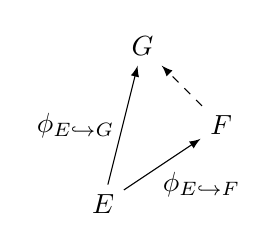
\begin{tikzpicture}
      \node (E) at (0, 0) {$E$}; 
      \node (F) at (1.5, 1) {$F$}; 
      \node (G) at (0.5, 2) {$G$}; 

      \draw[arrow] (E) -- (F);
      \draw[arrow] (E) -- (G);
      \draw[dashed-arrow] (F) -- (G);

      \node (f12) at (1.25, 0.25) {$\embed{E}{F}$};
      \node (f13) at (-0.35, 1) {$\embed{E}{G}$};
    \end{tikzpicture}

  \caption{An uncomplete diagram.}
  \label{fig:uncomplete}
\end{figure}

Let $E$, $F$, and $G$ be finite fields with
$\partial(E)\,|\,\partial(F)$ and
$\partial(F)\,|\,\partial(G)$. We also assume that $E\emb F$ and $E\emb G$,
hence we are in the situation described by Figure~\ref{fig:uncomplete}
where we miss one embedding. In order to complete the diagram of this
figure, Bosma,
Cannon and Steel suggest to take an arbitrary embedding $\embed{F}{G}'$ and to
``correct'' it by composing $\embed{F}{G}'$ with an element of
$\sigma\in\Gal(G/\mathbb{F}_p)$ such that 
\[
  \embed{E}{G}=\sigma\circ\embed{F}{G}'\circ\embed{E}{F}.
\]
We can then set $\embed{F}{G}=\sigma\circ\embed{F}{G}'$ and the
obtained embedding is compatible by construction. We also see that once we have
one compatible embedding, we can derive other compatible embeddings from it by
precomposing by an element $\xi$ of $\Gal(F/E)$. Indeed, such an element
$\xi$ fixes the elements in $E$, hence the compatibility conditions are
still verified after precomposition. One may wander what happens
if there are several subfields $E_1, \dots, E_r$, or if the configuration is not
the one presented in Figure~\ref{fig:uncomplete}.

There are three configurations with triangles, that are the one in
Figure~\ref{fig:triangles}. We already discussed the configuration on the
left, which is the one in Figure~\ref{fig:uncomplete}. The configuration in the
middle is easier to handle because we can set 
\[
  \embed{E}{G}=\embed{F}{G}\circ\embed{E}{F}
\]
since we have $E\emb F\emb G$. Finally, we will see later that the
configuration on the right cannot happen in the framework we use because on the
conditions we impose on the finite fields and on the embeddings betweem them.
  \begin{figure}
    \centering
    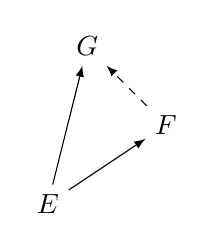
\begin{tikzpicture}
      \node (E) at (0, 0) {$E$}; 
      \node (F) at (1.5, 1) {$F$}; 
      \node (G) at (0.5, 2) {$G$}; 

      \draw[arrow] (E) -- (F);
      \draw[arrow] (E) -- (G);
      \draw[dashed-arrow] (F) -- (G);
    \end{tikzpicture}
    \phantom{and}
    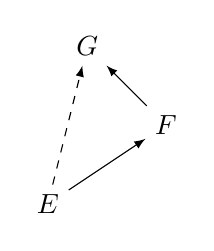
\begin{tikzpicture}
      \node (E) at (0, 0) {$E$}; 
      \node (F) at (1.5, 1) {$F$}; 
      \node (G) at (0.5, 2) {$G$}; 

      \draw[arrow] (E) -- (F);
      \draw[dashed-arrow] (E) -- (G);
      \draw[arrow] (F) -- (G);

    \end{tikzpicture}
    \phantom{and}
    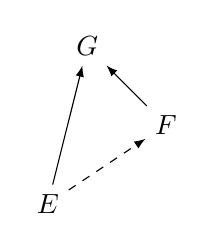
\begin{tikzpicture}
      \node (E) at (0, 0) {$E$}; 
      \node (F) at (1.5, 1) {$F$}; 
      \node (G) at (0.5, 2) {$G$}; 

      \draw[dashed-arrow] (E) -- (F);
      \draw[arrow] (E) -- (G);
      \draw[arrow] (F) -- (G);

    \end{tikzpicture}
    \caption{The different configurations with triangles.}
    \label{fig:triangles}
  \end{figure}

If we have a pair $\mathfrak L=(L, \Phi)$, where
$L$ is a set of finite fields and $\Phi$ is a set of embeddings between
elements of $L$, we say that $\mathfrak L$ is a \emph{lattice of compatibly
embedded finite fields} if
\begin{enumerate}
  \item[CE1] (unicity) for each pair $(E, F)$ of elements in $L$, there exists
    at most one corresponding embedding $\embed{E}{F}\in\Phi$.
  \item[CE2] (reflexivity) For each $E\in L$, the identity map
    $\Id_E=\embed{E}{E}$ is in $\Phi$.
  \item[CE3] (prime subfield) There is exactly one $P\in L$ such that $\partial
    (P) = 1$, and for all $F\in L$, there exists $\embed{P}{F}\in\Phi$
  \item[CE4] (invertibility) If $E\emb F$ and $\dE=\dF$, then $F\emb E$ and
    $\embed{F}{E}=\embed{E}{F}^{-1}$.
  \item[CE5] (transitivity) For any triple $(E, F, G)$ of elements in $L$, if $E\emb
    F\emb G$ then $E\emb G$ and
    $\embed{E}{G}=\embed{F}{G}\circ\embed{E}{F}$.
  \item[CE6](intersections) For each $E, F, G\in L$ such that $F\emb G$ and
    $E\emb G$, there exists $S\in L$ such that $\partial(S)=\gcd(\dE, \dF)$
    and $S\emb E$, $S\emb F$.
\end{enumerate}
These conditions are, for most of them, very natural. The condition CE3 is
technical and does not imply any work in our implementation because
finite fields elements in Nemo/Flint~\cite{Nemo, Flint} are represented by
polynomials over $\mathbb{F}_p$, so the embedding of $\mathbb{F}_p$ into an
extension is trivial. Finally, condition
CE6 ensures that the implicit isomorphisms between subfields are made
explicit.

Under those conditions, we can prove~\cite{BCS97} that we are able to add a finite field in
$L$ or an embedding that is not yet in $\Phi$ without altering the compatibility
of the lattice $\mathfrak L$.

\section{Implementation in Nemo}
\label{sec:implem}
In practice, we do not compute our embeddings by correcting random embeddings as
suggested in Section~\ref{sec:bcs-framework}. Instead, we use the naive
algorithm to compute a compatible embedding that does not need any correction.
Assume we are in the situation of Figure~\ref{fig:uncomplete}, \ie we have $E$,
$F$, $G$ finite fields and $E\emb F$, $E\emb G$, $\dF\,|\,\dG$. Let $\alpha_F$
be a generator of $F$ over $\mathbb{F}_p$, then $\alpha_F$ is also a generator
of $F$ over $E$. Let $\pi_{E}(\alpha_F)$ be the minimal polynomial of $\alpha_F$
over $E$, and let $\rho$ be a root of $\embed{E}{G}(\pi_E(\alpha_F))$, the
minimal polynomial of $\alpha_F$ viewed in $G$. We set $\embed{F}{G}$ to the
embedding mapping $\alpha_F$ to $\rho$. More precisely, we set
\[
  \embed{F}{G}(\sum_{i=0}^{[F:E]-1}e_i\alpha_F^i) =
  \sum_{i=0}^{[F:E]-1}\embed{E}{G}(e_i)\rho^i,
\]
hence we see that
\[
  \embed{E}{G} = \embed{F}{G}\circ\embed{E}{F}
\]
and the new embedding is compatible with the already existing ones. We take
the cannonical generator of $F$ over $\mathbb{F}_p$ to be $\alpha_F$, we compute
$\pi_E(\alpha_F)$ using linear algebra and we compute $\embed{F}{G}$ using
linear algebra too. Assume now that we have several finite fields $E_1, \cdots, E_r$ such
that for all $j$, $E_j\emb F$, $E_j\emb G$ and $\dF\,|\,\dG$. This is the
situation of Figure~\ref{fig:uncomplete-sev}.
\begin{figure}
  \centering
    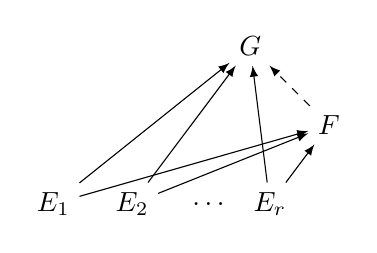
\begin{tikzpicture}
      \node (E1) at (-2, 0) {$E_1$}; 
      \node (E2) at (-1, 0) {$E_2$}; 
      \node (Er) at (0.75, 0) {$E_r$}; 
      \node (F) at (1.5, 1) {$F$}; 
      \node (G) at (0.5, 2) {$G$}; 
      \node (p) at (0, 0) {$\dots$};

      \draw[arrow] (E1) -- (F);
      \draw[arrow] (E1) -- (G);
      \draw[arrow] (E2) -- (F);
      \draw[arrow] (E2) -- (G);
      \draw[arrow] (Er) -- (F);
      \draw[arrow] (Er) -- (G);
      \draw[dashed-arrow] (F) -- (G);
  \end{tikzpicture}
  \caption{An uncomplete diagram with several subfields.}
  \label{fig:uncomplete-sev}
\end{figure}
In that case, we consider the polynomial
\[
  P = \gcd_i(\embed{E_i}{G}(\pi_{E_i}(\alpha_F))),
\]
and we let $\rho$ be a root of $P$. We see that $\rho$ is a root of each
polynomial $\embed{E_i}{G}(\pi_{E_i}(\alpha_F))$, so the embedding mapping
$\alpha_F$ to $\rho$ is compatible with all the previously existing embeddings.

\section{Conclusion}

In practice, because of condition CE6 concerning intersections, we might have to
compute additionnal embeddings before computing the wanted embedding. In
conclusion, in order to embed a finite field $F$ in $G$, we have to:

\begin{enumerate}
  \item for each subfield $S$ of $G$, check if the finite field $S\cap F$ is 
    embedded in $S$ and $F$, and if not, embed it. In practice, if there is not
    any finite field of degree $d=\gcd(\partial(S), \dF)$, we compute an
    arbitrary finite field $I$ of degree $d$ using Flint
    and we embed $I$ in $S$ and $F$.
  \item Embed $F$ in $G$ using Section~\ref{sec:implem} procedure.
  \item Compute the ``transitive closure'' of the lattice, \ie compute the
    embeddings such that condition CE5 holds. In practice we compute all the
    embeddings and keep them in memory.
\end{enumerate}
The first step implies a recursive call to our embedding algorithm, so the
complexity of the operation might explode at that step.

There are several things that could be enhanced in our current framework. First,
we could use graph algorithms in order to compute the transitive closure only
when asked by the user. We could also compute minimal polynomials using
Berlekamp Massey algorithm instead of linear algebra.

\bibliographystyle{plain}
\bibliography{erou}
\end{document}
